\documentclass{article}

% preamble.tex source: Templates for CCSC Conferences (paper_template)
% https://github.com/ccsc-journal/ccsc-editor/tree/master
\input{preamble}

\addbibresource{paper.bib}

%path to figures - \usepackage{graphicx} is included in preamble.tex
\graphicspath{{figures/}}

\title{Audio Clustering via Community Detection on a kNN Graph of Audio Embeddings\footnote{CSCI 693 Research Methods in Computer Science, Spring 2026}}

\author{
  Hannah Tiffany\affmark[1]\\
  \affmark[1]Computer Science\\
  California State University, Chico\\
  Chico, CA 95929\\
  \email{\{student,hltiffany\}@csuchico.edu}
}

\begin{document}
\maketitle

\begin{abstract}
  This research explores how graph clustering can be used for audio sample grouping. Audio signals are embedded to feature space using the CLAP neural network. The cosine similarity between audio samples is used to determine a similarity value between audio embeddings, based on harmonics, frequency, and structure. From this data, a kNN graph is constructed, with edges connecting the k=5 and 10 most similar audio samples. Community detection is achieved via the Leiden algorithm to group nodes together that are most densely connected by their edges. The results of this paper show that community detection has the potential to be an effective way to determine classification groups and create the basis of a GNN. Additionally, adjusting the k-value was found to be a method of adjusting the level of discrimination in the clustering. At k=5, more communities and more divisive clustering occurred, while a higher k produced fewer, more generalized communities.
\end{abstract}


\section{Introduction}
Classifying audio signals is a complex problem that continues to be the subject of research. This research project aims to add to this field by using clustering algorithms on a kNN graph of embedded audio to group together similar embeddings. The goal of this project is to research how well these clusters will group together audio with the same label.

\subsection{Context and Background}
Audio classification and genre detection are ongoing areas of research. Machine learning has shown great benefits in improving audio classification. One method is through embeddings. Contrastive Language-Audio Pretraining (CLAP) \cite{elizalde} is one such transformer. CLAP is trained on 128,000 audio samples and their textual descriptions. Audio samples are decomposed into their spectral components and embedded via an audio encoder. The textual description is embedded with a text encoder, and the two are joined together in multi-modal space via linear projection. This research uses the angle between vectors to quantify a similarity value between the corresponding audio samples. A graph can be constructed from these embeddings, where each node represents an audio sample, and edges represent the cosine similarities between them. 

To perform classification, groups of similar audio signals must be determined. This is achieved with Leiden clustering \cite{traag}. The Leiden clustering algorithm defines communities as groups of nodes that are more densely connected to each other than to nodes outside, as measured by modularity. The algorithm uses heuristics to try to identify the split that maximizes modularity. The algorithm is composed of three main phases:
\begin{enumerate}[noitemsep]
  \item Local Moving of Nodes: Nodes are initially assigned to individual clusters, then moved between clusters to maximize modularity.
  \item Refinement of Partitions: The internal structure of each community is refined to ensure no disconnected nodes.
  \item Aggregation into Super-nodes: The network's structure is simplified by aggregating the nodes in each community into one super-node.
\end{enumerate}
For this paper, the third step is ignored. A super-node is most helpful when trying to aggregate similar nodes together into one large node. Analyzing the quality of the communities is an important piece of this research, which is not easily accomplished through a super-node. It does not make sense to form a super-node for this research, as it would need to be decomposed again for analysis purposes. 

\subsection{Problem Statement and Research Question}
The goal of this research is to use graph clustering for the purpose of audio grouping. This research will answer the question: "How well can graph clustering find groups of similar audio samples, as measured by modularity, the silhouette coefficient, and the Davies-Bouldin score?" 

\subsection{Significance of the Study}
This paper is impactful in how it uses graphs and audio embedding for audio grouping. This work could have future applications in genre detection, identifying similar songs, or classifying audio as speech, music, or environmental sound. It could also serve as the base for a Graph Neural Network to classify audio.

\subsection{Scope and Organization}
The next section of this paper will summarize the current literature available in this field. Next, the methodology of this study will be explained, including the research design and data collection methods. Finally, the results and implications of the study will be summarized. 

\section{Literature Review}
  The field of audio classification has been researched for many years. Most recently, the field has made significant strides by leveraging machine learning techniques. The benefit of using graph properties to improve classification, either by representing individual audio samples as a graph or through classification on a graph composed of samples, has also been explored.

Early work tried to classify audio signals by finding similar patterns across samples. 
In 2002, Lie Lu et al. presented a method for audio classification as speech, 
music, environmental sound, or silence by looking for patterns within the signal \cite{lu}.
This paper has two goals: to classify the type of audio and, if the audio is speech,
segment speech audio based on the speaker. The paper uses the K-Nearest Neighbors (kNN) 
algorithm is applied to the zero-crossing rate of a frame to differentiate between different 
types of samples. Speech signals often display a pattern of alternating voiced and unvoiced 
sounds that music signals do not, which can be identified by the kNN. Silence can be determined 
by an average short-time energy and a zero-crossing rate lower than a given threshold. 
Discriminating music and environmental sounds can be achieved with band periodicity, spectrum 
flux, and noise frame ratio. Segmentation is achieved using Linear Spectral Pairs to 
discriminate between two speakers. The final results found that this method worked well for 
discriminating between music, speech, and environmental noises. Speaker discrimination worked 
fairly well, but struggled to detect the same speaker in different environments.

 The rise of machine learning provided significant contributions to multiple fields, including audio classification. C. Aironi et al. combined machine learning with graphs to develop an approach that could uncover features that were missed with simple signal analysis and pattern detection \cite{Aironi}. Developed in 2021, this approach derives the graph from the log-Mel scale spectrogram. Two classification methods are performed, one with a GNN and one with a CNN+GNN combination. Although the model performed worse than a state-of-the-art CNN designed for audio classification, the results showed that the graph embedding was able to capture important underlying features that were otherwise missed. This showed promise for potential future work and the benefit of utilizing graphs.

An additional area of research is zero-learning, in which a model must classify data from categories that were not present in the testing data by using auxiliary features. In 2021, Xie et al. compared semantic embeddings of audio classes with audio embeddings to match zero-shot data with a class description \cite{Xie}. A compatibility function is used to compare how similar an audio embedding and a semantic embedding are. The results showed that this method performed better than random guessing and was significantly improved by including cases that are semantically close to the test cases in the training stage. This model worked so well that it became the inspiration and basis for the CLAP encoder used in this dataset.

More recently, neural networks, which can capture more complex structures of the sample, have been used to show an improvement in classification over signal inspection techniques. In 2024, A. E. Castro-Ospina et al. explored a graph-based neural network for the task of audio classification \cite{castro-ospina}. The proposed methodology uses pre-trained models designed to extract deep features from audio files, which are used as the nodes of the graph. The audio is mapped to feature space using the three embedding strategies, VGGish, PANN, and YAMNet. A kNN graph is constructed by creating an edge from each embedding to its kNN nearest neighbors. Three GNNs were used on the graph to classify the audio: GCN, GraphSAGE, and GAT. The results showed that graphs are a very useful way to extract audio information and that GNNs obtain competitive performance in audio classification.

Genre classification, which focuses on music samples, is a difficult research question based on the subjectivity of genre determination. In 2024, Ding et al. used a novel machine learning technique to demonstrate superiority over existing genre classification methods \cite{ding}. A knowledge graph is built that embeds relationships between genres, artists, and instruments. The knowledge graph is novel for its use of two branches: the audio branch for extracting features from the original audio, and the KG branch to extract knowledge-aware features. Using a model inspired by Node2Vec, the knowledge graph is used to classify an audio signal based on where it falls in the feature space.

\section{Methodology}

\subsection{Research Design}
This research is an experimental study to classify sound through graph community detection. The nodes of the graph will be composed of \textit{i} audio samples, $a_i$. Audio samples are sourced from FreeSound and Free Music Archive, which house open-source audio samples available for download. For this research, audio, speech, and environmental sounds were used. Each audio sample is represented by a feature vector $z_i$, which comprises the node features. 

Feature vectors are learned through audio embedding via CLAP, a pre-trained neural network for audio to vector embedding. Using a pretrained neural network was determined to be the best choice for this project, because building and developing a new neural network is not the focus of the research and is outside the scope of the project. Simpler methods, which do not require a neural network, were considered, such as the log-mel spectrogram averaged over time, but this would not be nearly as robust. An audio embedding from a neural network gives the best representation of the audio sample by capturing timbre, texture, semantic similarity, and some temporal structure. It is also less sensitive to noise, time shifts, and small spectral variations. CLAP was chosen over other models because it was trained on large audio datasets containing multiple different kinds of audio, including the three used in this project (speech, environmental sounds, and music). It is a good choice for similarity detection because it also learns and embeds semantic similarity.

A kNN graph is built by connecting each audio sample to its top k nearest neighbors, evaluated on cosine similarity. Cosine similarity measures the angle between vectors, which represents similarity between audio embeddings. Magnitude is often arbitrary and noisy; thus is not a necessary measurement. For this project, which focuses on small graphs, the values of k will be 5 and 10. Edges will only be added if they have a similarity score in the top 70\% of calculated scores. Preliminary research showed that, on average, the bottom 30\% of edges added did not reflect a meaningful cosine similarity. Therefore, they were removed. This limits the number of edges between nodes that are dissimilar from the rest of the dataset. 

After the graph is built, the Leiden Algorithm is used for community detection to determine audio clusters from the graph. Each audio signal is labeled prior to the embedding with the correct classification. After the graph is built and communities are detected, the silhouette coefficient and adjusted random index are calculated as measures of the strength of the clustering.

Two datasets are used in this research. The first contains a mix of 29 audio signals, broken down as follows: 10 speech, 7 singing (without music), 11 instrumental music, and one constant tone. The second set contains music of five different genres: pop, country, rock, hip-hop, and R\&B. Five songs for each genre are included. Community detection with a k value of 5 and 10 was performed for each dataset. Values of 5 and 10 were chosen to cover lower and higher ratios of nodes to edges, 0.2/1 and 0.4/1 nodes per edge. This will explore how different ratios of edges will impact the communities found. For this research, labels for communities are not predicted and assigned to the clusters. This could be accomplished using CLAP and is a possible area of future work. Due to the lack of predicted labels, intrinsic metrics are used to evaluate the quality of the clusters, which do not require a prediction label. Three metrics are evaluated in this paper:

\begin{enumerate}[noitemsep]
  \item Modularity: Measures the strength of division of the network by measuring the weight of edges within the cluster versus out of the cluster. The Leiden algorithm clusters nodes by maximizing modularity. Values above 0.3 often indicate more internal edges than random chance. A value above 0.7 is rarely achieved on real-world graphs.
  \item Silhouette Coefficient\cite{rousseeuw}: Measures how well a point fits in its cluster when compared to other clusters. It is calculated with the mean intra-cluster distance and the mean nearest-cluster distance for each sample. Values range from -1 to 1, with higher scores indicating better clustering. A score above 0.5 would indicate strong clusters, while scores below 0.25 would show poor clustering without substantial structure.
  \item Daives-Bouldin Score\cite{davies}: Measures the average similarity of each cluster with its most similar cluster, where similarity is measured as the ratio of within-cluster distances to between-cluster distances. The DB score gives insight into the between-cluster separation. Lower scores indicate better separation. Values between 0 and 1 are considered high-quality scores, while 1-2 show fair clustering with some overlap. Values above 2 suggest poor and unreliable clustering.
\end{enumerate}

\section{Results}

\subsection{Summary of Findings}
Table \ref{table:nonlin} compares the effectiveness of the clustering from each graph. It should be noted that the Leiden algorithm is a heuristic algorithm, and therefore, there is some amount of randomness involved in the communities it detects after each run. The algorithm was run 10 times for each of the following datasets, and the highest-scoring split is used for these results. The best scores were achieved by the mixed dataset with k=5. Since this dataset is composed of mixed audio samples, the different communities are easier to differentiate because their embeddings have a larger difference in cosine similarity when compared to the music sample.
The first three tests have statistically significant results that imply the resulting community splits were not found due to random chance, according to their modularity and Davies-Bouldin scores. The last test, music with k=10, has a modularity of 0, meaning no communities could be determined. This test also reports a very poor silhouette coefficient and Davies-Bouldin score, which indicate poor clustering and structure. This is likely because of the high connectedness of the graph. For this dataset, only 5 samples of each genre were used, so the remaining 5 edges were forced onto more dissimilar audio samples. The cosine similarities are closer than those of the mixed audio dataset, so the separation between audio groups becomes less pronounced. This made community detection difficult because there are no obvious groups of nodes with "in" edges and "out" edges. 

\begin{table}[ht]
\caption{Clustering Effectiveness per Graph} % title of Table
\label{table:nonlin} % is used to refer to this table in the text
\centering % used for centering table
\resizebox{\textwidth}{!}{%
\begin{tabular}{c c c c c c} % centered columns (4 columns)
\hline\hline %inserts double horizontal lines
Graph & \# Audio Types & \# Detected Communities & Modularity & Silhouette Coefficient & DB Score \\ [0.5ex] % inserts table
%heading
\hline % inserts single horizontal line
Mixed, k=5 & 4 & 3 & 0.5112 & 0.1290 & 1.532  \\ % inserting body of the table
Mixed, k=10 & 4 & 2 & 0.3215 & 0.1261 & 1.553 \\
Music, k=5 & 5 & 4 & 0.3711 & 0.0012 & 2.493 \\
Music, k=10 & 5 & 1 & 0 & -0.009 & 2.576\\ [1ex]
\hline %inserts single line
\end{tabular}
}
\end{table}

\subsection{Mixed Dataset}

Figure \ref{fig:mixed5Heatmap} shows the heatmap of cosine similarities between audio embeddings for the dataset of mixed audio. The heatmap groups the embeddings with the most similar cosine similarities together. Speech signals are labeled "sp", singing as "si", music as "ms", and the tone as "to".
Three clear groups can be found from this map. From the top left, the first includes six of the speech samples. The second, grouped closely to speech, includes six of the singing samples. The third has the remaining speech samples.
A final group can be seen appearing at the bottom right, composed of the music samples. This cluster effect shows that the embedding is working as expected, and can effectively plot audio in higher dimensions well enough that cosine similarity can detect a noticeable difference.
\begin{figure}[htbp]
  \centering
  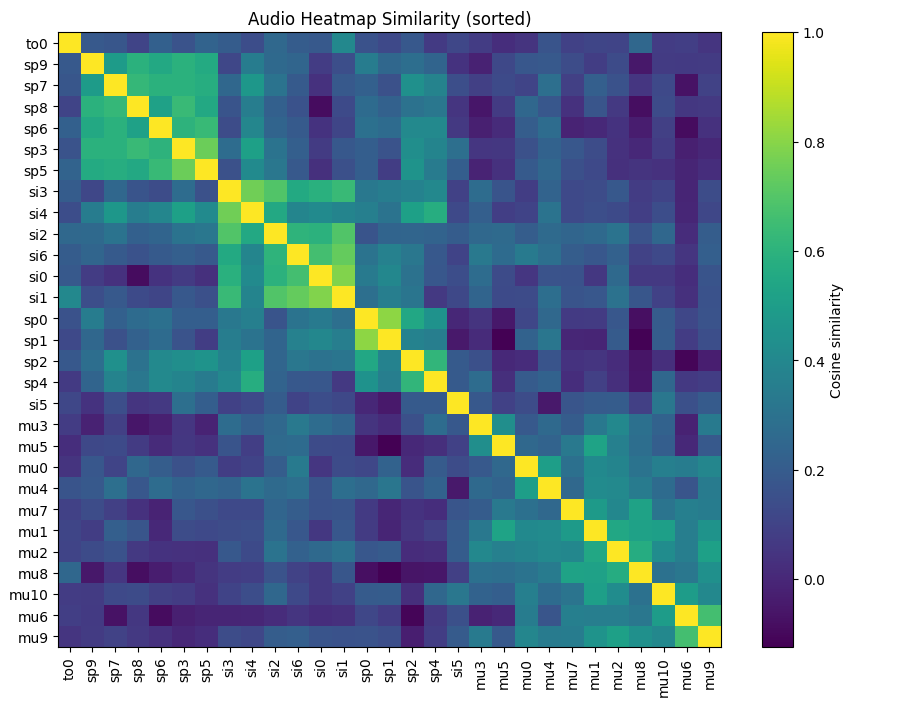
\includegraphics[width=\linewidth]{mixed5Heatmap}
  \caption{Heatmap of cosine similarities between audio embeddings on the mixed dataset, where k=5}
  \label{fig:mixed5Heatmap}
\end{figure}


Figure \ref{fig:mixed5} below shows the graph created from the mixed signals dataset at k=5. Nodes of the same type of audio signal are colored the same. This figure shows the ground truth of community clusters.
\begin{figure}[htbp]
  \centering
  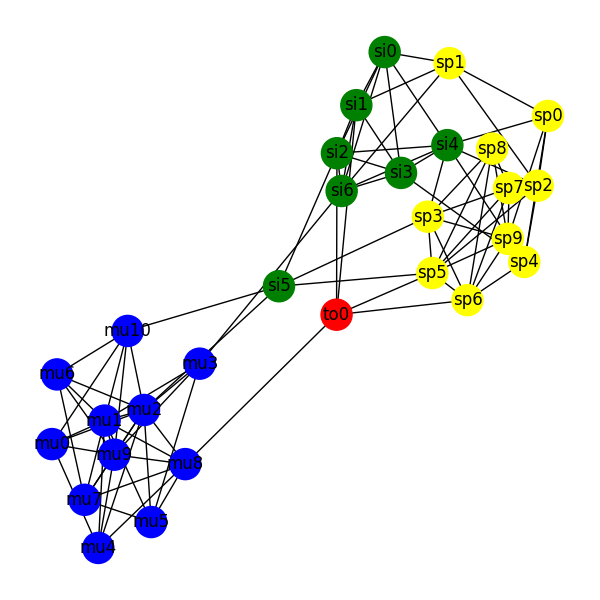
\includegraphics[width=\linewidth]{mixed5}
  \caption{Graph of mixed audio signals dataset, k=5}
  \label{fig:mixed5}
\end{figure}
Figure \ref{fig:mixed5communities1} below shows the best cluster separation achieved from this graph. The seperation shows three distinct communities, which mirror the heatmap. The yellow community contains the six speech signals that were clustered at the top right on the heatmap. The blue community contains a mix of singing and speech audios, which contain the second and third group on the heatmap, as well as the singular tone. It can be seen on the graph that even though four of the speech signals are grouped with the singing, they also contain edges to the other speech signals, while the singing samples have edges that connect to music samples. The single tone sample sits in the middle, with edges to each group. The purple group contains all ten music samples, with one singing sample. 
The communities found by the clustering algorithm mirror the ones visually discernible from the heatmap. This is noteworthy because it shows how the community clustering is working in line with the embedding. Audio that is embedded together in feature space can be discovered by the Leiden clustering algorithm.
\begin{figure}[htbp]
  \centering
  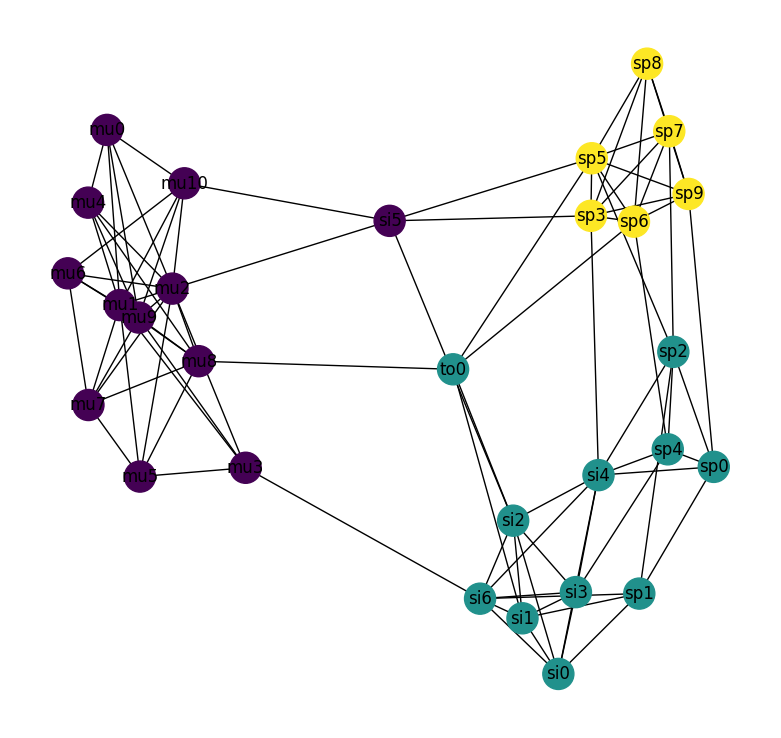
\includegraphics[width=\linewidth]{mixed5communities1}
  \caption{Detected communities from the mixed audio dataset, k=5}
  \label{fig:mixed5communities1}
\end{figure}

Figure \ref{fig:mixed10} below shows the graph created from the mixed signals dataset at k=10. Nodes of the same type of audio signal are colored the same. This is the ground truth communities for this graph.
\begin{figure}[htbp]
  \centering
  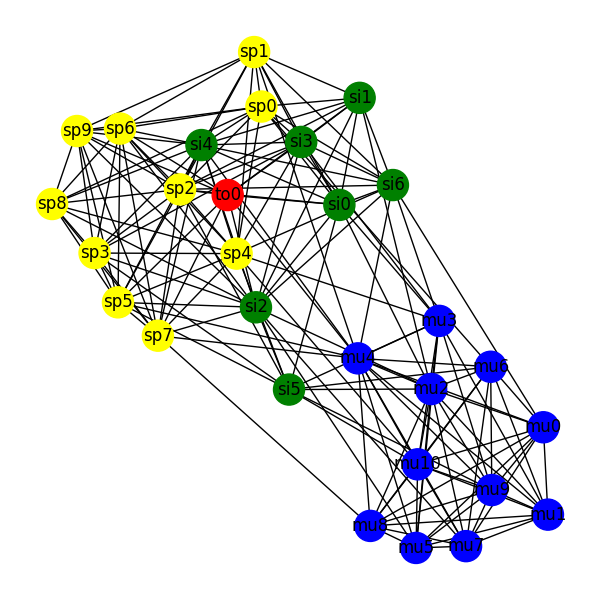
\includegraphics[width=\linewidth]{mixed10}
  \caption{Graph of mixed audio signals dataset, k=10}
  \label{fig:mixed10}
\end{figure}

Figure \ref{fig:mixed10communities1} below shows the best clustering achieved from this graph. This clustering makes a clear distinction between music samples and vocal samples. The purple cluster contains the music samples, and the yellow cluster contains the singing and speech samples. This follows the communities detected in the heatmap, but with less detail. The distinct line that can be visually discerned between "si1" and "sp0" is detected by this community grouping. From these results, it can be seen that a higher value of k, as it relates to the ratio of nodes to edges, will result in community detection that shows finer detail in community detection. Increasing the k value will create more generalized communities, which reflect very different types of audio.
\begin{figure}[htbp]
  \centering
  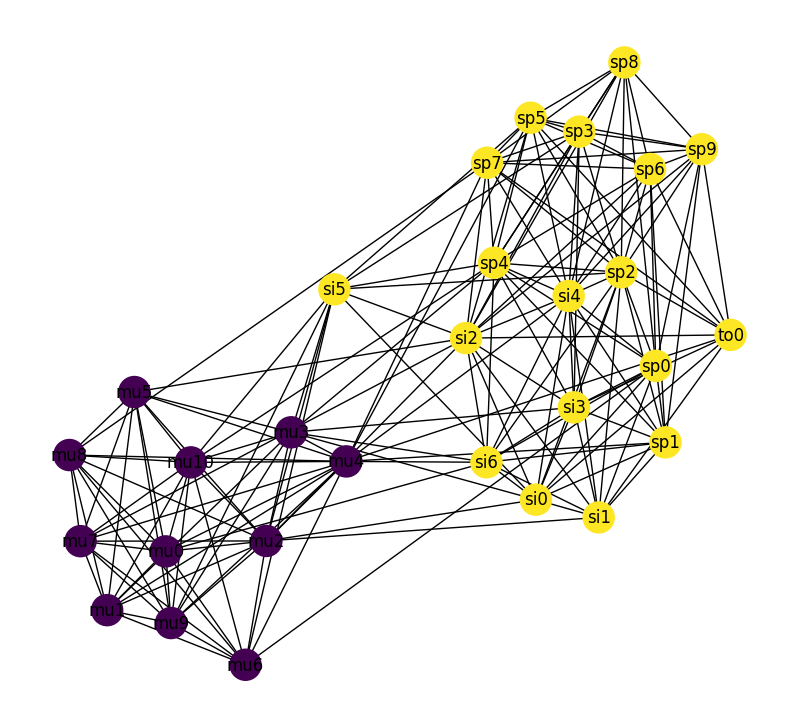
\includegraphics[width=\linewidth]{mixed10communities1}
  \caption{Detected communities from the mixed audio dataset when k=10}
  \label{fig:mixed10communities1}
\end{figure}

\subsection{Music Dataset}

Figure \ref{fig:music5Heatmap} shows the heatmap of cosine similarities between audio embeddings. The heatmap is sorted by grouping together the most similar audio embeddings based on cosine similarity. Rock is labeled "ro", pop as "po", hip-hop as "hi", country as "co", and R\%B as "rn". This heatmap shows less clear groupings than the mixed audio dataset. Two clear groupings appear in the bottom right and towards the middle left of the image, but there is no clear pattern or genre similarity from the audio in these groupings. Again, these results show that the embedding is effective for detecting splits, although less so than with the mixed audio dataset. Although clear groups can be observed visually, it is not apparent that they follow patterns of a similar genre. This shows that the embedding is weaker for different music genres, and the cosine similarity is less effective. These results are to be expected, since the CLAP model used in this research was trained on a dataset containing a wide range of audio and is not optimized for music.
\begin{figure}[htbp]
  \centering
  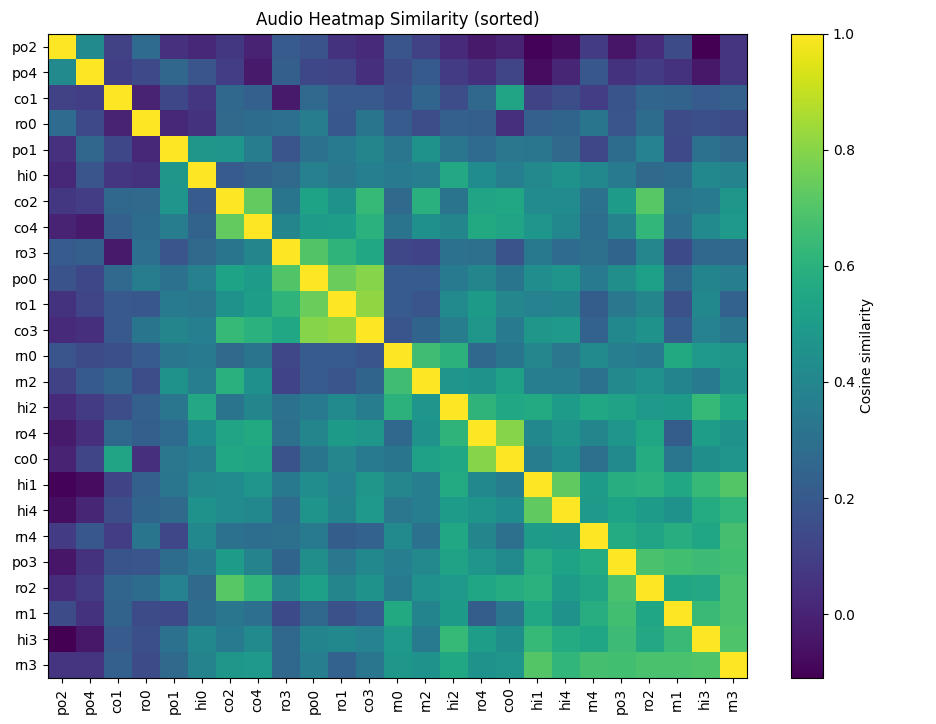
\includegraphics[width=\linewidth]{music5Heatmap}
  \caption{Heatmap of the cosine similarity of the music dataset, k=5}
  \label{fig:music5Heatmap}
\end{figure}

Figure \ref{fig:music5} below shows the graph created from the music samples dataset when k=5. Nodes are colored by genre. This is the ground truth of communities.
\begin{figure}[htpb]
  \centering
  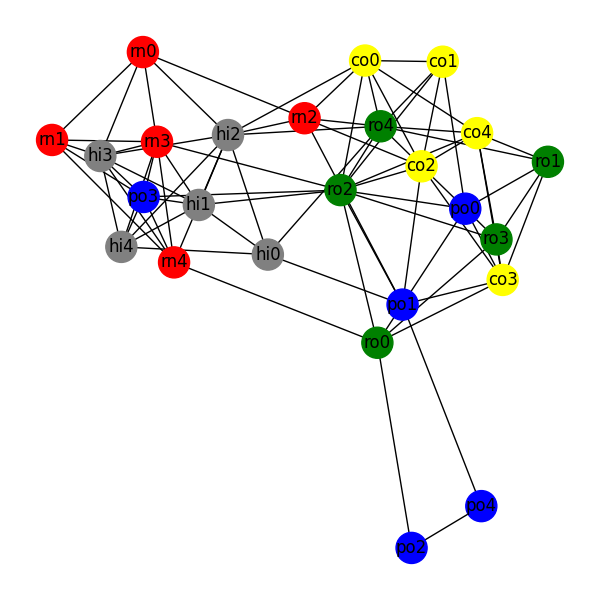
\includegraphics[width=\linewidth]{music5}
  \caption{Graph of music audio signals dataset, k=5}
  \label{fig:music5}
\end{figure}

Figure \ref{fig:music5communities2} shows the best detected clustering of music genres when k=5. Some patterns from the heatmap persist in this graph, but genre groupings do become slightly more apparent.
Hip-hop and R\&B are grouped together in the blue community. Country and rock are sorted together in the green community. The yellow community makes up a collection of pop, rock, and country. Finally, the purple community is composed of two pop songs, which were sorted as the most dissimilar from other audio by the heatmap.
As with the mixed audio dataset, the clustering follows the patterns discovered in the heatmap. However, it does a better job of grouping the audio into similarity categories than are immediately obvious when looking at the raw similarity values or observing the heatmap. As an example, R\&B and hip-hop were grouped together at one end of the graph. This result is not surprising, because hip-hop was born out of rapping over R\&B beats. They often have very similar production styles and beats. This pattern is observed again, as rock and country are grouped together in the middle of the graph. From observing the heatmap or raw embeddings, these groupings are not clear. Graph community detection acts as a method of making these splits more apparent. 
\begin{figure}[htbp]
  \centering
  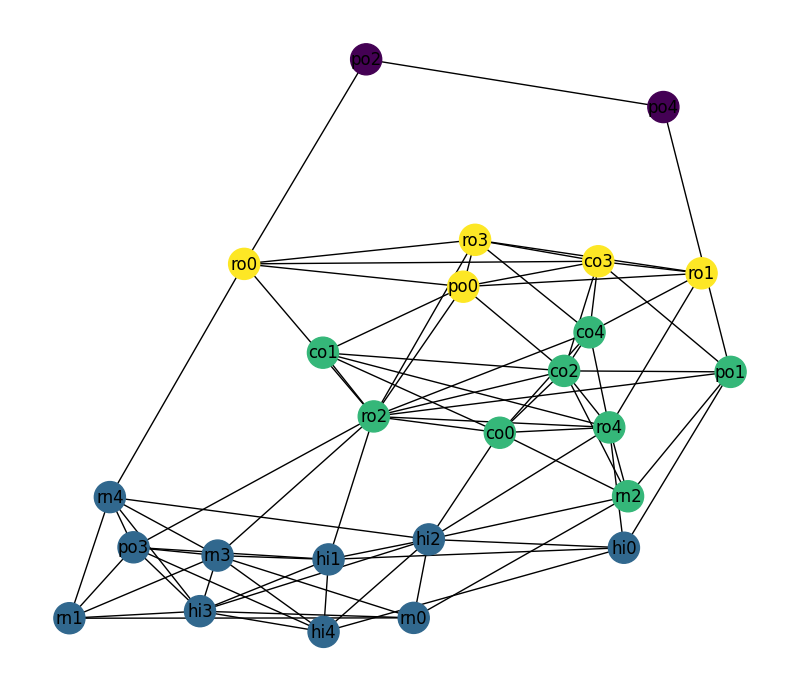
\includegraphics[width=\linewidth]{music5communities2}
  \caption{Communities detected from the music genre dataset when k=5.}
  \label{fig:music5communities2}
\end{figure}

Figure \ref{fig:music10} below shows the graph created from the music genres dataset at k=10. Nodes are colored by genre. This is the ground truth for these communities.
\begin{figure}[htbp]
  \centering
  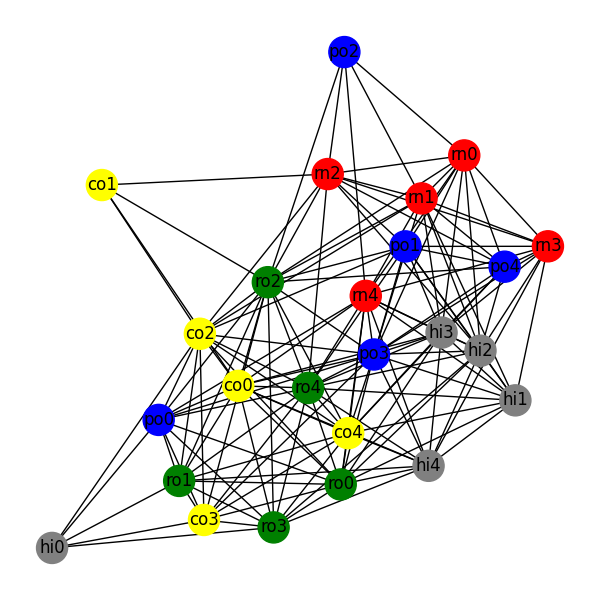
\includegraphics[width=\linewidth]{music10}
  \caption{Graph of music genres dataset, k=10}
  \label{fig:music10}
\end{figure}

Figure \ref{fig:music10communities1} below shows the only clustering that the Leiden algorithm was able to detect across the 10 runs. This graph was too dense to split into communities, therefore only one community is detected. These results show the importance of finding the ideal k value for the dataset and the communities of interest. A higher k value, as determined by the ratio of nodes to edges, appears ineffective in a case where the audio is of the same type (i.e., all music).
\begin{figure}[htbp]
  \centering
  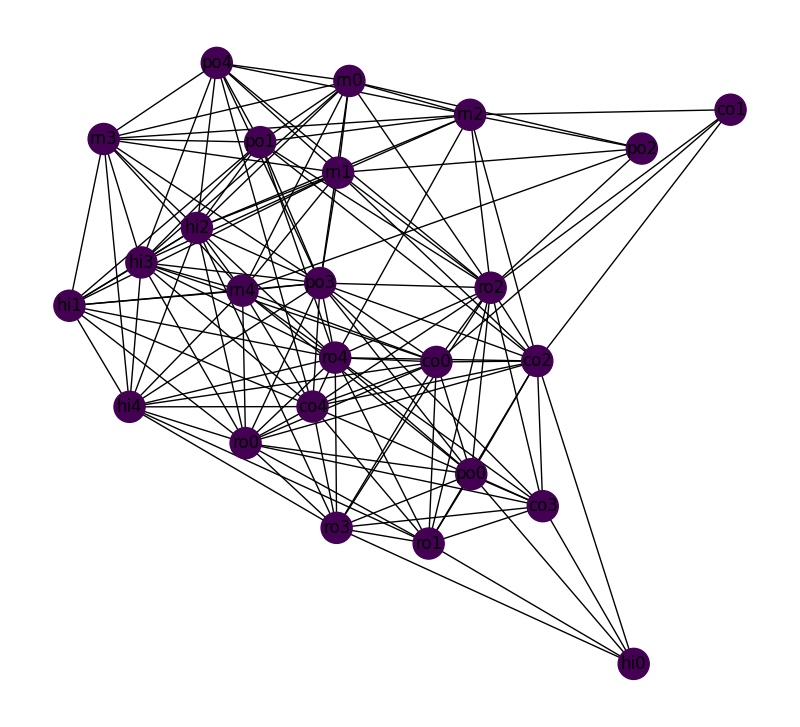
\includegraphics[width=\linewidth]{music10communities1}
  \caption{Communities detected from the music genres dataset at k=10}
  \label{fig:music10communities1}
\end{figure}

\subsection{Key Observations}
Community detection shows the ability to reflect the cosine similarities discovered by the heatmap, but also reveals patterns that are not at first obvious. Graphs that exhibit the most clear clustering are made from datasets that contain are very different elements from each other, such as speech and music. Communities become less accurate and more difficult to detect as the audio becomes more similar. A higher k value will result in a more general differentiation (i.e., speech versus music), while a lower k value will reveal more nuanced details (i.e., different genres). This reveals the importance of selecting a k value that considers the number of nodes, the type of dataset, and the types of communities to be detected.

\section{Discussion}

\subsection{Interpretation of Results}
This research reveals that graphs can be an effective tool for genre classification. The patterns observed in the heatmap became more apparent and amplified as the audio was graphed and clustered. The graph provided a "sliding scale" of audio types, shifting from one type to another throughout the graph, with the most dissimilar audio types on opposite ends.

The mixed audio dataset grouped speech and music on opposite ends. This is expected, as speech and music often take on very different spectral representations. Singing was placed in between, leaning closer to speech, but with the rhythmic elements of music samples. These patterns are discovered by the audio embedding and revealed in the graph structure. 
With a k value of 5, a modularity score of 0.5112 is achieved, reflecting a successful and significant community structure. However, the silhouette coefficient remained very low, at 0.1290. This is indicative of poor clustering, without substantial structure. However, it should be noted that a high silhouette score becomes more difficult to achieve on a small dataset with similar embeddings. This explains why the silhouette score remains low, despite the modularity achieving a high value. Additionally, the Leiden algorithm aims to maximize modularity, so it would be expected to be the best value out of the three. The Davies-Bouldin score of 1.532 balances the two and shows fair community detection, but still some overlap between clusters. This appears to be the most accurate with what can be visually observed from the graph.
When the k value increases to 10, the scores become slightly worse. Modularity decreases to 0.3215. This is to be expected, as a greater number of edges leads to more edges between communities. The silhouette coefficient and Davies-Bouldin score remain similar, at 0.1261 and 1.553. This reflects a decent community grouping, but not perfect, with some significant overlap between separate communities. Overall, it appears that using graph community detection on the mixed audio dataset performs fairly well, but not perfectly.

The community detection on the music dataset showed the advantage of being able to distinguish patterns that are not easy to see from raw data. R\&B and hip-hop were grouped together at one end of the graph. Towards the middle of the graph, rock and country act as a bridge to the other far extreme of the graph, which contains two heavy, electronic pop songs, which . These songs sound very dissimilar to the red of the dataset, because they were the edges trimmed by the threshold. In between
this community and the rock/country community, there is a "transition" community of mainly pop and rock. The heavier pop songs are connected to this community through heavy rock songs. This graph provides an interesting view of genre as not a binary classification, but instead a spectrum. Although songs may be different genres, such as R\&B and hip-hop, the graph structure reveals similarities between them that are backed up by the historical factors of these genres. 

\subsection{Implications}
These results have implications in the field of audio classification and music detection. By leveraging graph properties, a more detailed picture of an audio sample can be painted. Audio classification is often not a binary decision, as audio signals are often composed of multiple different parts (ie, singing and instrumental music, and music sample which takes inspiration of multiple genres, etc.) Graphing these signals can reveal patterns and connections that may not be obvious by simply looking at a single value.

\subsection{Limitations}
This study was greatly limited by a small sample size. It is difficult to draw conclusions from two small datasets. One other limitation of this study was the community detection algorithm selected. The Leiden algorithm works by maximizing modularity, which is computed based on the ratio of edges "in" the community versus edges "out" of the community. However, modularity can suffer from the "resolution limit", in which the maximum modularity often fails to detect smaller communities. Modularity is often considered a decent heuristic, but not the best tool for finding community splits. Additionally, each node is forced to have k edges, forcing some edges to be added to somewhat dissimilar audio signals, especially for samples that are
unique, or when the k-value exceeds the number of samples in a given community. This is handled slightly by the threshold, which removes the bottom 30\% of edges, but it may be more effective to determine a constant value that the cosine similarity must reach before an edge is added between two nodes. This may remove more
"out" edges, and may be an effective way to separate audio that is similar but should still be in different communities (ie, speech and singing).

\subsection{Suggestions for Future Research}
The first step to expand this research is to collect more audio samples. Additionally, it would be beneficial to dive deeper into the exact audio signals and why they were grouped where. For example, examining the signal structure of an incorrectly classified sound, or listening to a music sample on the edge of two communities to determine if it might fit into both.

It would also be beneficial compared to another metric, such as the Mel-frequency cepstral coefficient, used to model human hearing, to numerically determine if audio that is grouped together sounds similar to the human ear.

The model for music dataset could also likely be improved by training the embedding for music specifically. In this project, CLAP was trained on a dataset containing a combination of music, speech, and environmental sounds. However, data containing only music can make the model more attuned to picking up features in music specifically and improve clustering based on genre.

Another interesting area of future research involves labeling the clusters for true audio classification. Currently, the songs are only grouped by similarity, but the type of audio in a community is not determined. However, CLAP can also be used to return a textual classification of the audio. A future area of research could use these labels to determine audio groups in the graph, and compared to the baseline.

Finally, determining a song's genre is often a difficult task, open to discretion and interpretation. Many songs fit into more than one category. This research grouped songs into only one genre, based on what is considered the dominating genre. However, labeling songs with a more nuanced view of genre (i.e., including multiple genres on one song, overlapping community detection, and identifying bridge songs) could provide extra explanations for the edges added and the communities detected.

\section{Conclusion}
The research explores the use of graphs as a method of audio classification. The results of this study show that graphs can reveal patterns between audio that are not immediately obvious, but expand upon the idea of audio classification as a binary task. Adding the step of community detection expands upon the embedding itself by finding splits and clusters within the embedding space. Although this project showed only moderate effectiveness, more research is required to determine how well graph clustering can perform on embedded audio.

This research adds to the field of audio classification by exploring a new method of finding similar audio samples. Audio and genre classification are important and rapidly evolving. This research shows that taking advantage of machine learning and graph theory can expand audio classification from a binary to a sliding scale.

Although this research was limited in its scope and size, expanding upon it could reveal interesting results. These methods could be used as a base for a Graph Neural Network to find songs that sound similar, strip vocals from music, determine the genres of a song, or group audio samples into similar groups.

\medskip

\printbibliography

\end{document}